\section {Frequentist properties of posterior probability for mass ordering}
\label{sec:mh}

We can consider the Bayesian posterior probability for the mass hierarchy from a frequentist perspective by looking at the distribution of mass ordering posterior probabilities for given true values of the mass ordering and \deltacp. This allows us to understand how often we make Type-I and Type-II errors for a given true mass ordering and true value of \deltacp for a particular threshold (chosen to be 95\%), given our current exposure.

The approach taken is to use the Feldman-Cousins toys to compute the value

\begin{equation}
	\text{P(NO)} = \frac{L_\text{NO}}{L_\text{NO} + L_\text{IO}}
\end{equation}

for each toy, where P(NO) is the posterior probability of the normal ordering hypothesis, $L_\text{NO}$ and $L_\text{IO}$ are the respective average likelihoods assuming normal and inverted ordering, averaged over all values of \deltacp, yielding a distribution of 20K posterior probabilities.

\subsection{Results for $\delta_{CP} = \pm\pi$}
In \cref{fig:mh_dcp_mpi} the mass ordering posterior probability distributions are shown with true $\delta_{CP} = \pm\pi$ in the case of each true mass ordering, while \cref{tab:mh_dcp_mpi} shows the probability of rejecting each mass ordering for a given true mass ordering.

\begin{figure*}[htb]
	\center
	\begin{subfigure}[b]{0.49\textwidth}
		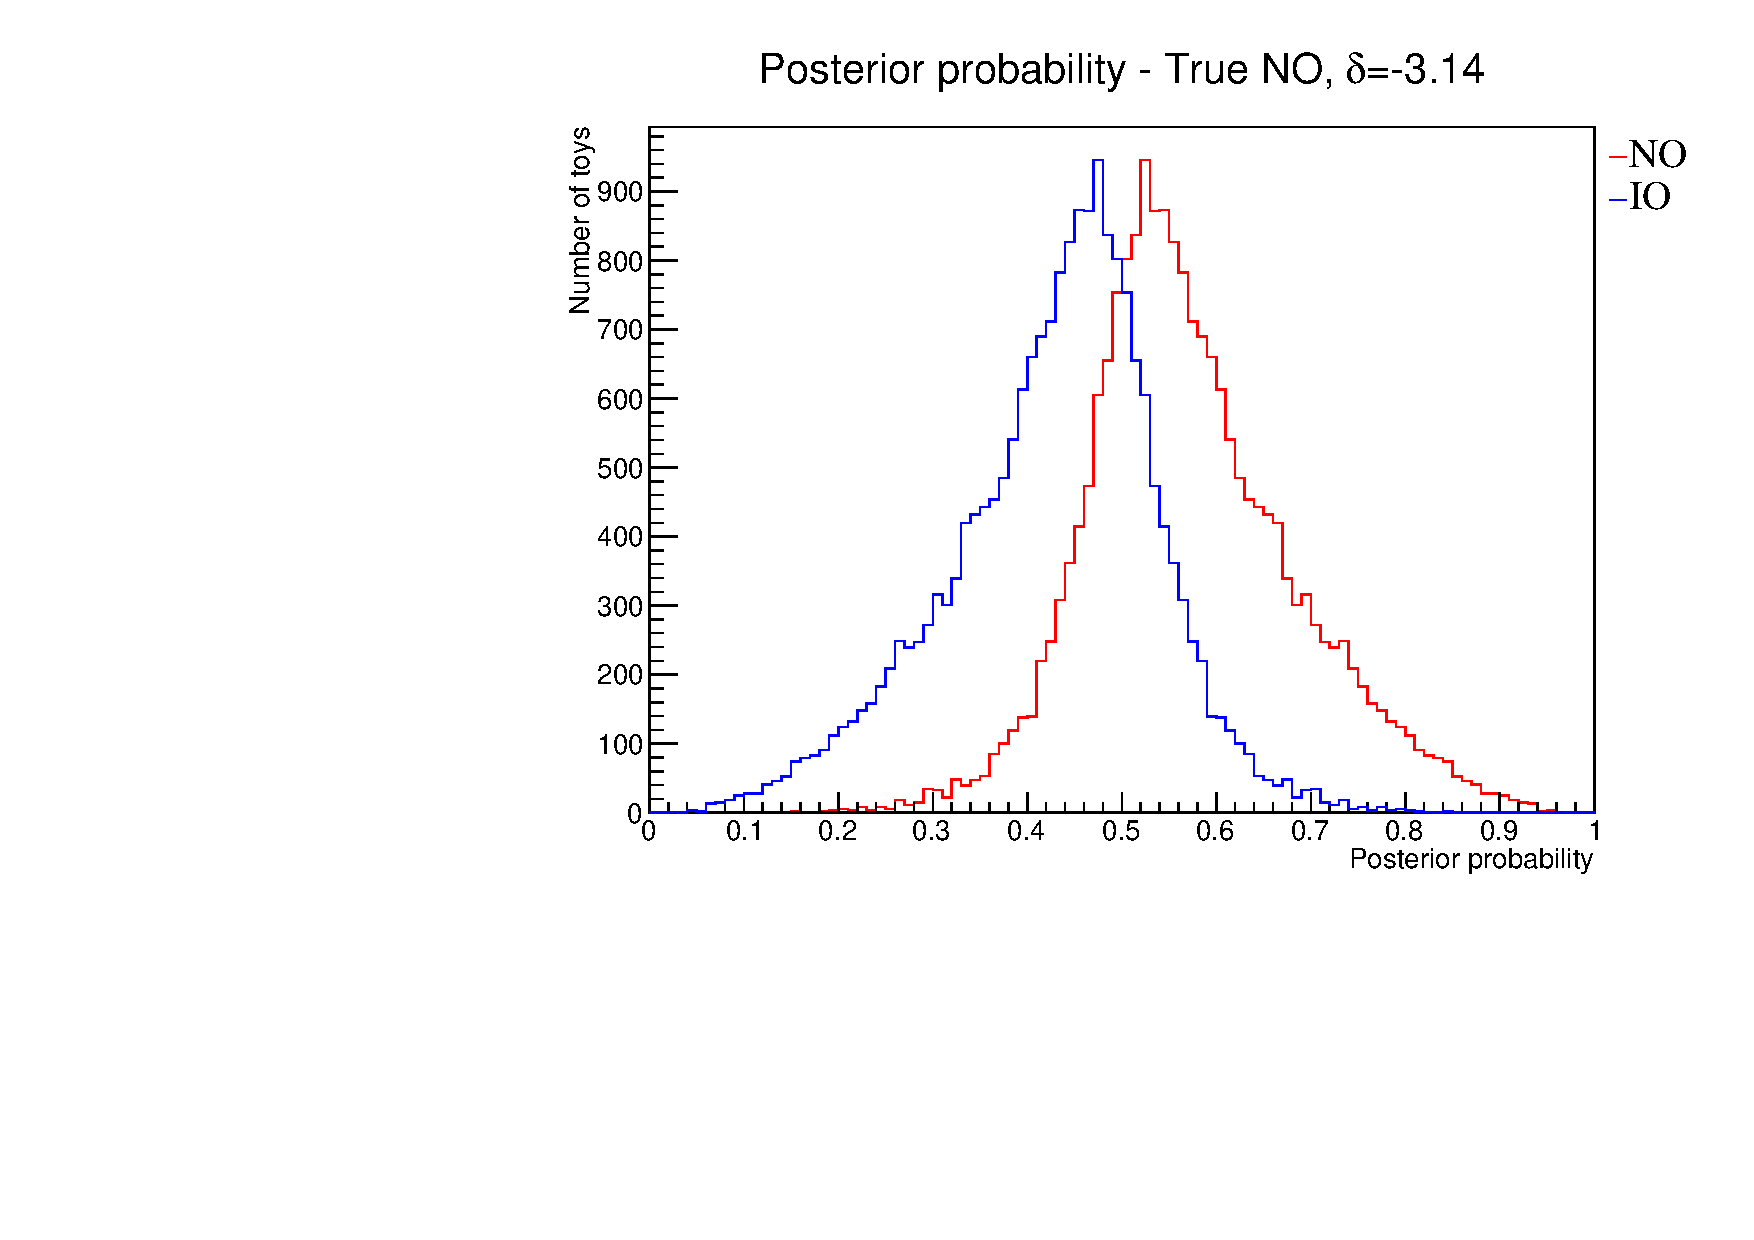
\includegraphics[width=0.9\textwidth, page=1]{images/mh/mh_posterior_mpi}
		\caption{True normal ordering}
	\end{subfigure}
	\begin{subfigure}[b]{0.49\textwidth}
		\includegraphics[width=0.9\textwidth, page=2]{images/mh/mh_posterior_mpi}
		\caption{True inverted ordering}
	\end{subfigure}
	\caption {
		Posterior probability distributions of the two mass orderings given $\delta_{CP} = \pm\pi$ and the true mass ordering.
	}
	\label{fig:mh_dcp_mpi}
\end{figure*}

\begin{table}[htb]
\centering
\begin{tabular}{| c | c | c |}
\hline
True ordering & Reject false ordering & Reject true ordering \\
\hline
Normal & 0.00020 & 0.00000 \\
Inverted & 0.00000 & 0.00000 \\
\hline
\end{tabular}

\caption{
The probability to reject the false and true mass orderings at 95\% threshold for the given true mass ordering.
}
\label{tab:mh_dcp_mpi}
\end{table}

It can be seen from \cref{tab:mh_dcp_mpi} that we have little sensitivity to the mass ordering for true $\delta_{CP} = \pm\pi$.

\FloatBarrier
\clearpage

\subsection{Results for $\delta_{CP} = -3\pi/4$}
In \cref{fig:mh_dcp_m3pi4} the mass ordering posterior probability distributions are shown with true $\delta_{CP} = -3\pi/4$ in the case of each true mass ordering, while \cref{tab:mh_dcp_m3pi4} shows the probability of rejecting each mass ordering for a given true mass ordering.

\begin{figure*}[htb]
	\center
	\begin{subfigure}[b]{0.49\textwidth}
		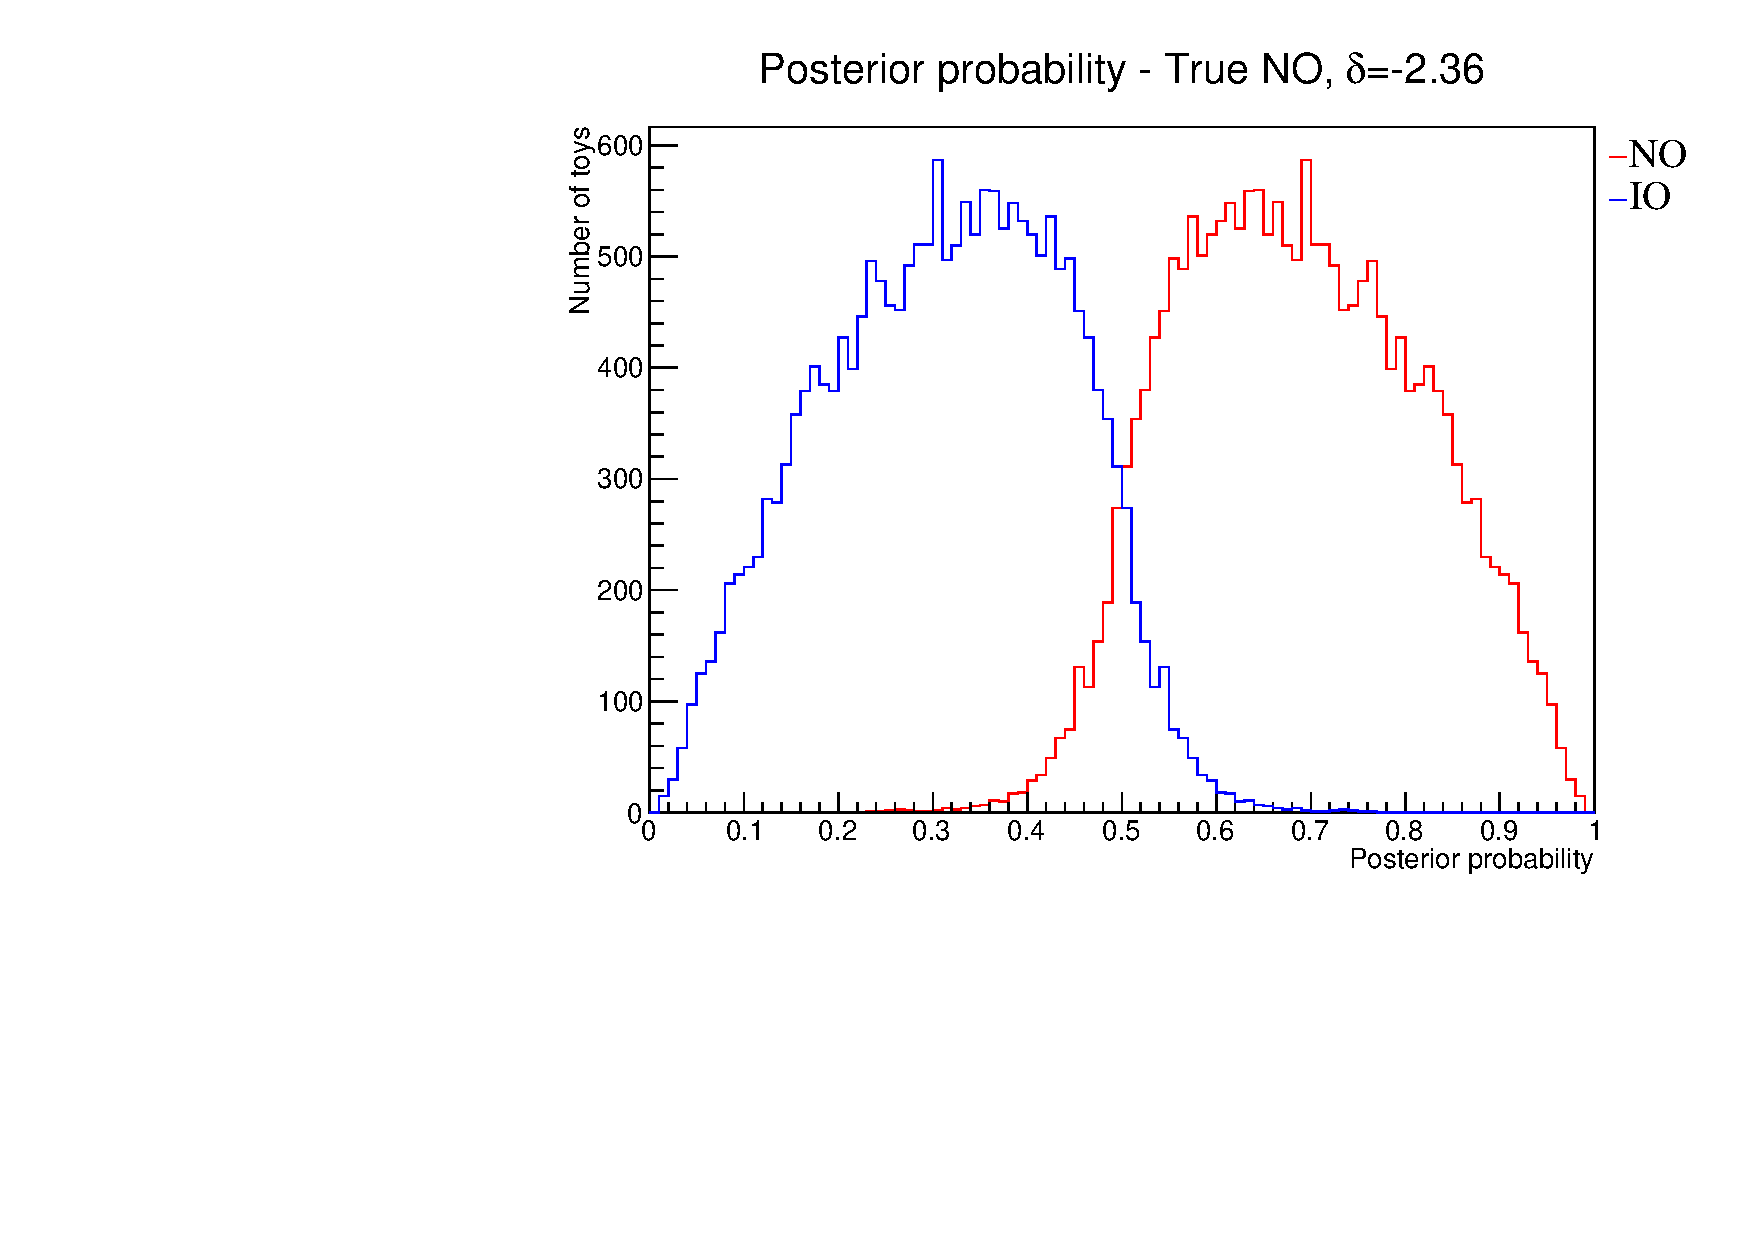
\includegraphics[width=0.9\textwidth, page=1]{images/mh/mh_posterior_m3pi4}
		\caption{True normal ordering}
	\end{subfigure}
	\begin{subfigure}[b]{0.49\textwidth}
		\includegraphics[width=0.9\textwidth, page=2]{images/mh/mh_posterior_m3pi4}
		\caption{True inverted ordering}
	\end{subfigure}
	\caption {
		Posterior probability distributions of the two mass orderings given $\delta_{CP} = -3\pi/4$ and the true mass ordering.
	}
	\label{fig:mh_dcp_m3pi4}
\end{figure*}

\begin{table}[htb]
\centering
\begin{tabular}{| c | c | c |}
\hline
True ordering & Reject false ordering & Reject true ordering \\
\hline
Normal & 0.01000 & 0.00000 \\
Inverted & 0.00000 & 0.00015 \\
\hline
\end{tabular}

\caption{
The probability to reject the false and true mass orderings at 95\% threshold for the given true mass ordering.
}
\label{tab:mh_dcp_m3pi4}
\end{table}

It can be seen from \cref{tab:mh_dcp_m3pi4} that we have little sensitivity to the mass ordering for true $\delta_{CP} = -3\pi/4$.

\FloatBarrier

\subsection{Results for $\delta_{CP} = -\pi/2$}
In \cref{fig:mh_dcp_mpi2} the mass ordering posterior probability distributions are shown with true $\delta_{CP} = -\pi/2$ in the case of each true mass ordering, while \cref{tab:mh_dcp_mpi2} shows the probability of rejecting each mass ordering for a given true mass ordering.

\begin{figure*}[htb]
	\center
	\begin{subfigure}[b]{0.49\textwidth}
		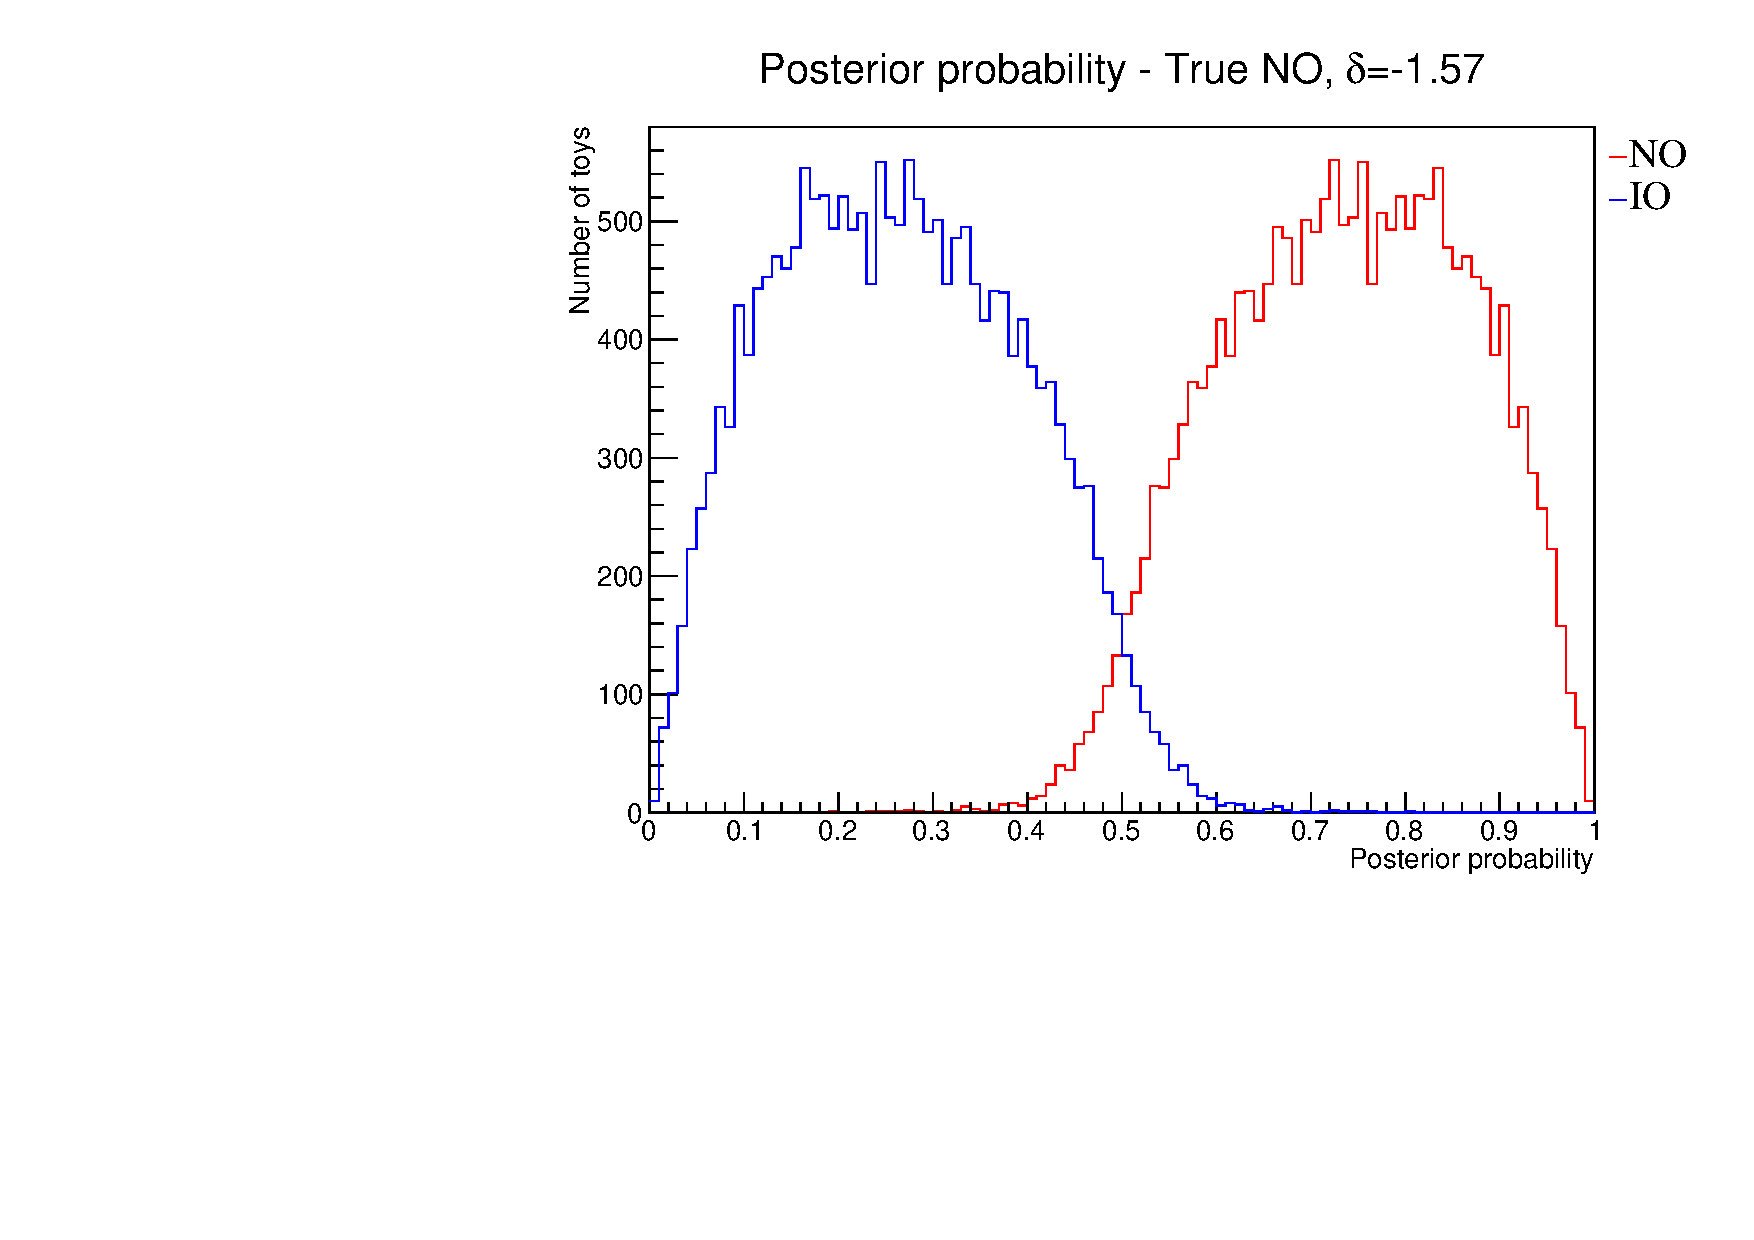
\includegraphics[width=0.9\textwidth, page=1]{images/mh/mh_posterior_mpi2}
		\caption{True normal ordering}
	\end{subfigure}
	\begin{subfigure}[b]{0.49\textwidth}
		\includegraphics[width=0.9\textwidth, page=2]{images/mh/mh_posterior_mpi2}
		\caption{True inverted ordering}
	\end{subfigure}
	\caption {
		Posterior probability distributions of the two mass orderings given $\delta_{CP} = -\pi/2$ and the true mass ordering.
	}
	\label{fig:mh_dcp_mpi2}
\end{figure*}

\begin{table}[htb]
\centering
\begin{tabular}{| c | c | c |}
\hline
True ordering & Reject false ordering & Reject true ordering \\
\hline
Normal & 0.02820 & 0.00000 \\
Inverted & 0.00000 & 0.00160 \\
\hline
\end{tabular}

\caption{
The probability to reject the false and true mass orderings at 95\% threshold for the given true mass ordering.
}
\label{tab:mh_dcp_mpi2}
\end{table}

It can be seen from \cref{tab:mh_dcp_mpi2} that only one hierarchy can be rejected for each given true hierarchy, and that in turn the rate at which we reject the true hypothesis is $\sim6\%$ of the rate at which we reject the false hypothesis ($\sim0.2\% / 2.8\%$), broadly consistent with our interpretation of posterior probability.

\FloatBarrier

\subsection{Results for $\delta_{CP} = -\pi/4$}
In \cref{fig:mh_dcp_mpi4} the mass ordering posterior probability distributions are shown with true $\delta_{CP} = -\pi/4$ in the case of each true mass ordering, while \cref{tab:mh_dcp_mpi4} shows the probability of rejecting each mass ordering for a given true mass ordering.

\begin{figure*}[htb]
	\center
	\begin{subfigure}[b]{0.49\textwidth}
		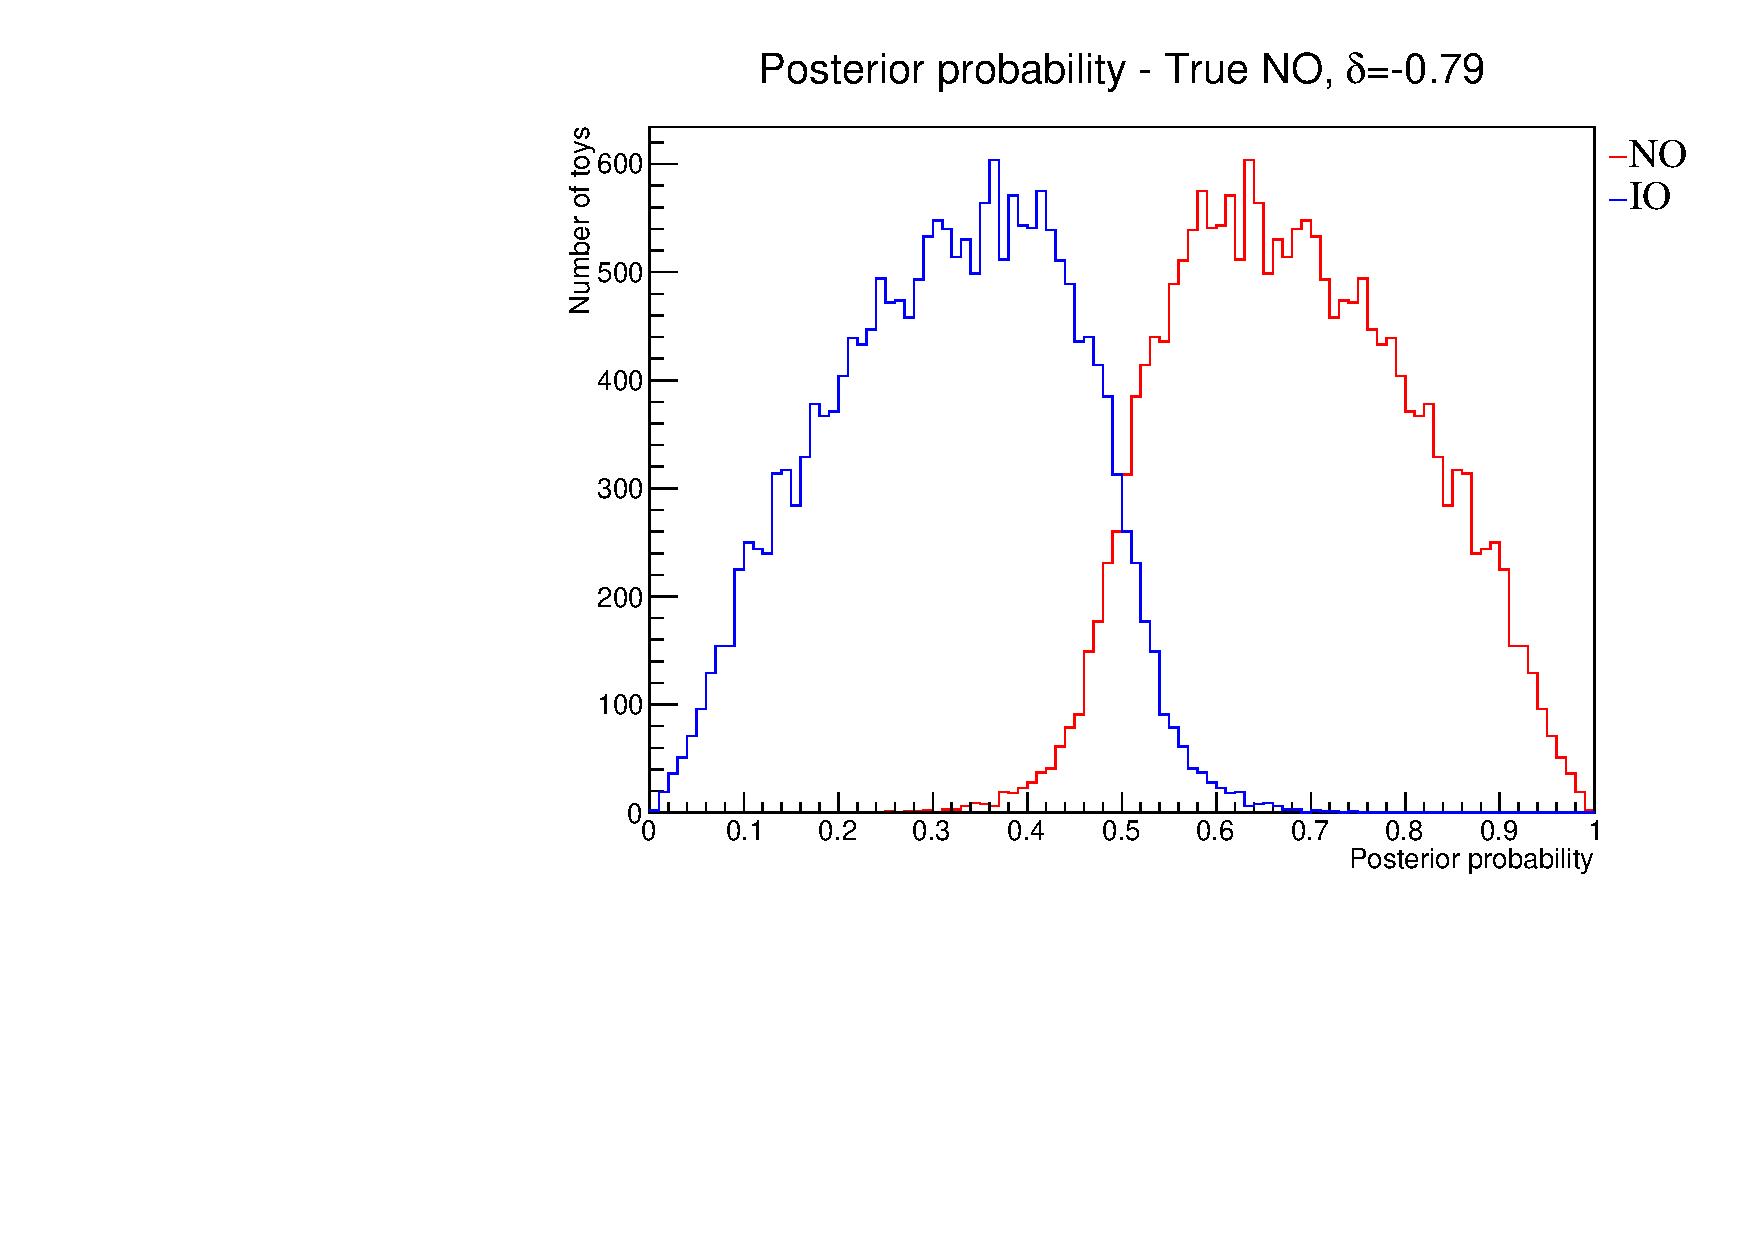
\includegraphics[width=0.9\textwidth, page=1]{images/mh/mh_posterior_mpi4}
		\caption{True normal ordering}
	\end{subfigure}
	\begin{subfigure}[b]{0.49\textwidth}
		\includegraphics[width=0.9\textwidth, page=2]{images/mh/mh_posterior_mpi4}
		\caption{True inverted ordering}
	\end{subfigure}
	\caption {
		Posterior probability distributions of the two mass orderings given $\delta_{CP} = -\pi/4$ and the true mass ordering.
	}
	\label{fig:mh_dcp_mpi4}
\end{figure*}

\begin{table}[htb]
\centering
\begin{tabular}{| c | c | c |}
\hline
True ordering & Reject false ordering & Reject true ordering \\
\hline
Normal & 0.00895 & 0.00000 \\
Inverted & 0.00000 & 0.00055 \\
\hline
\end{tabular}

\caption{
The probability to reject the false and true mass orderings at 95\% threshold for the given true mass ordering.
}
\label{tab:mh_dcp_mpi4}
\end{table}

It can be seen from \cref{tab:mh_dcp_mpi4} that we have little sensitivity to the mass ordering for true $\delta_{CP} = -\pi/4$.

\FloatBarrier

\subsection{Results for $\delta_{CP} = 0$}
In \cref{fig:mh_dcp_0} the mass ordering posterior probability distributions are shown with true $\delta_{CP} = 0$ in the case of each true mass ordering, while \cref{tab:mh_dcp_0} shows the probability of rejecting each mass ordering for a given true mass ordering.

\begin{figure*}[htb]
	\center
	\begin{subfigure}[b]{0.49\textwidth}
		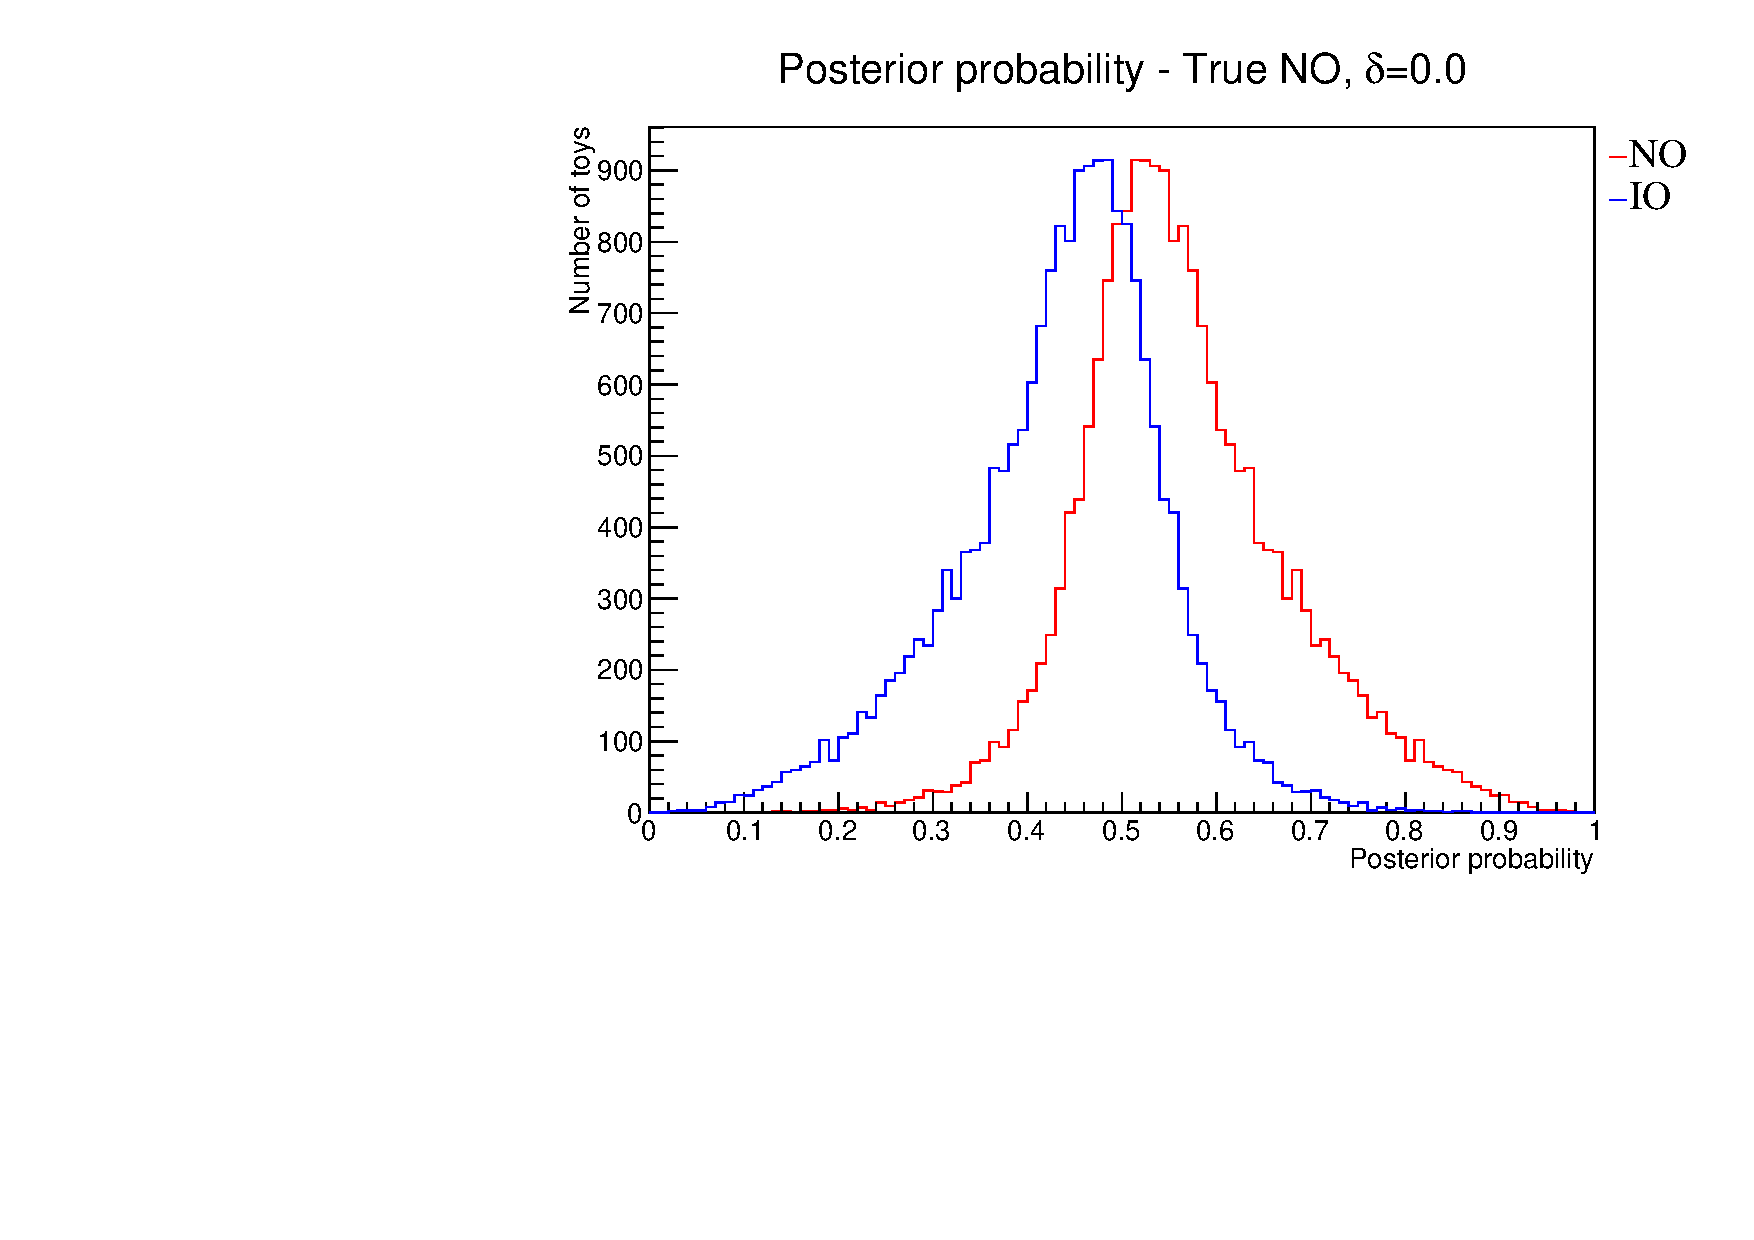
\includegraphics[width=0.9\textwidth, page=1]{images/mh/mh_posterior_0}
		\caption{True normal ordering}
	\end{subfigure}
	\begin{subfigure}[b]{0.49\textwidth}
		\includegraphics[width=0.9\textwidth, page=2]{images/mh/mh_posterior_0}
		\caption{True inverted ordering}
	\end{subfigure}
	\caption {
		Posterior probability distributions of the two mass orderings given $\delta_{CP} = 0$ and the true mass ordering.
	}
	\label{fig:mh_dcp_0}
\end{figure*}

\begin{table}[htb]
\centering
\begin{tabular}{| c | c | c |}
\hline
True ordering & Reject false ordering & Reject true ordering \\
\hline
Normal & 0.00040 & 0.00000 \\
Inverted & 0.00005 & 0.00000 \\
\hline
\end{tabular}

\caption{
The probability to reject the false and true mass orderings at 95\% threshold for the given true mass ordering.
}
\label{tab:mh_dcp_0}
\end{table}

It can be seen from \cref{tab:mh_dcp_0} that we have little sensitivity to the mass ordering for true $\delta_{CP} = 0$.

\FloatBarrier

\subsection{Results for $\delta_{CP} = +\pi/4$}
In \cref{fig:mh_dcp_ppi4} the mass ordering posterior probability distributions are shown with true $\delta_{CP} = +\pi/4$ in the case of each true mass ordering, while \cref{tab:mh_dcp_ppi4} shows the probability of rejecting each mass ordering for a given true mass ordering.

\begin{figure*}[htb]
	\center
	\begin{subfigure}[b]{0.49\textwidth}
		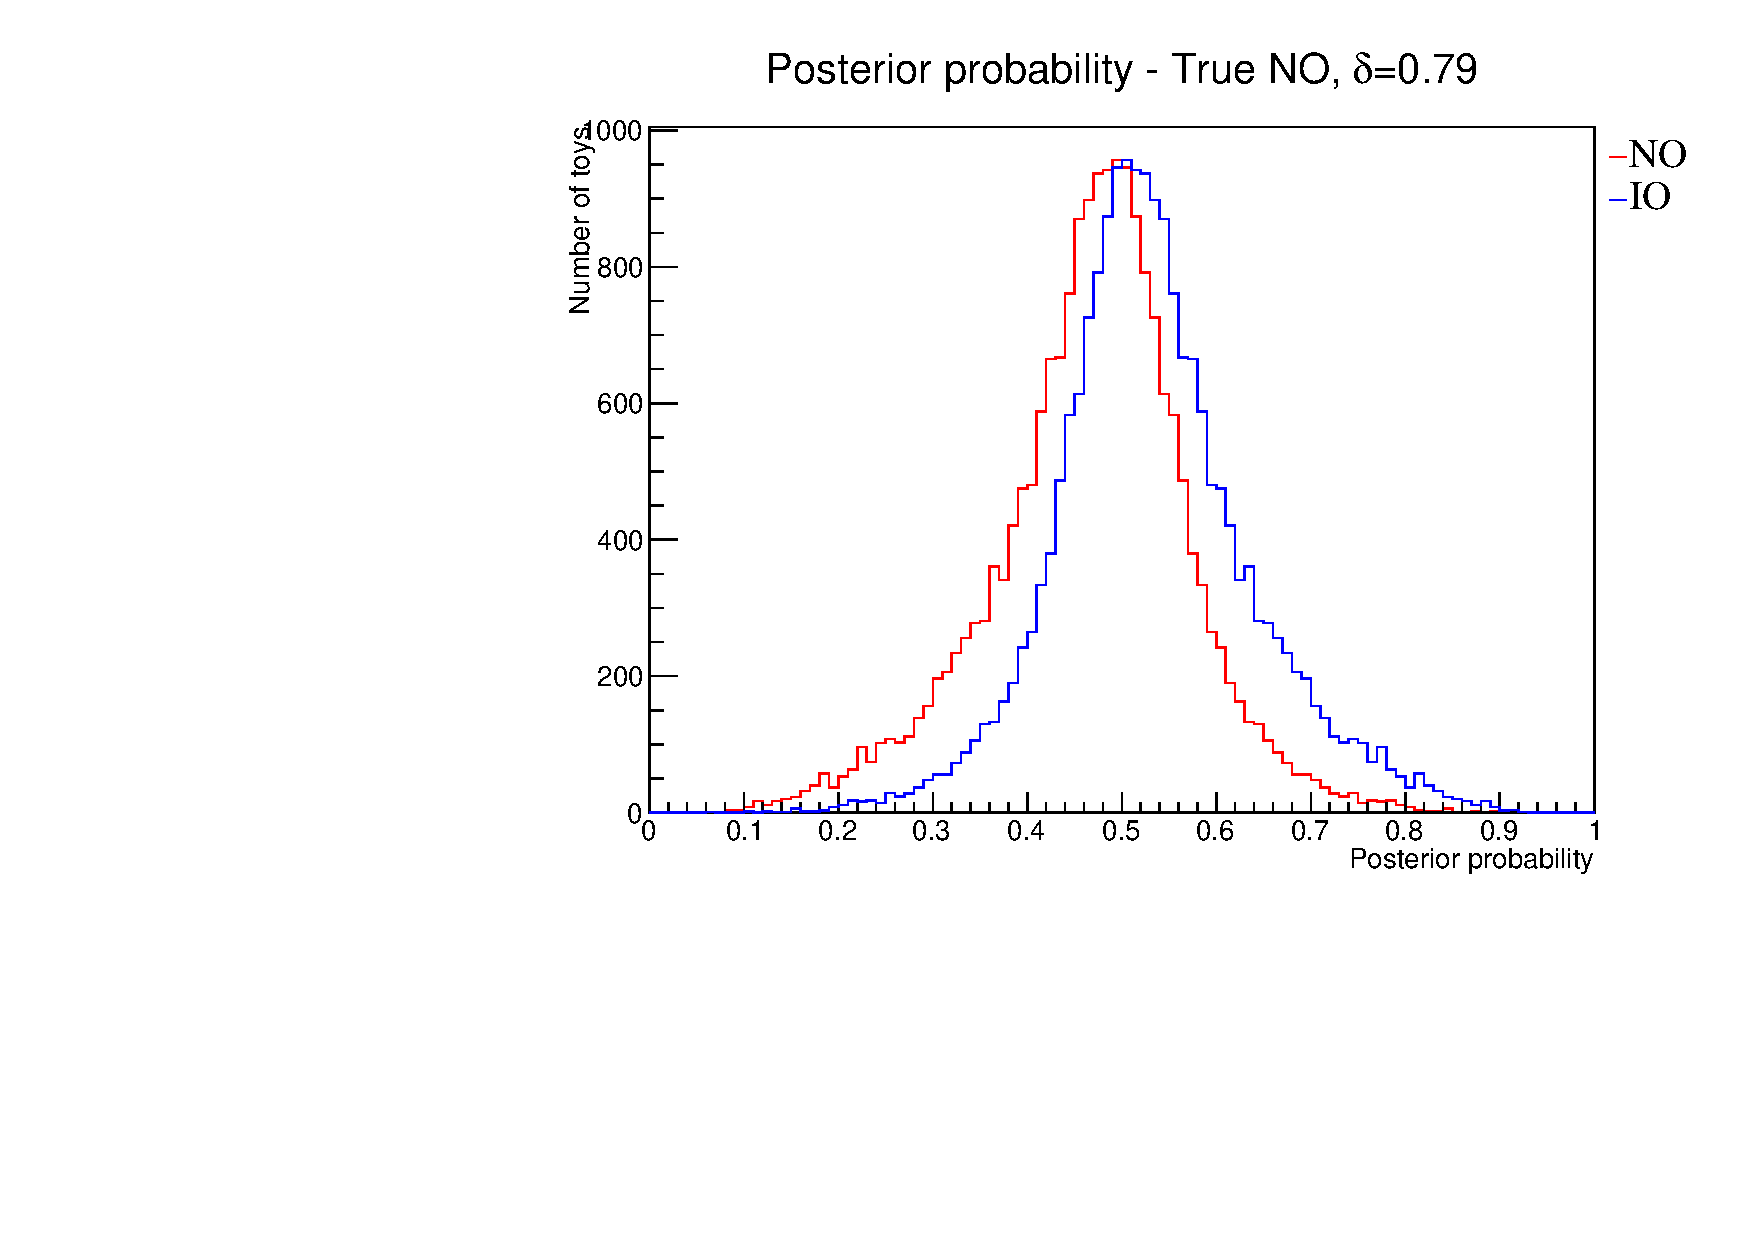
\includegraphics[width=0.9\textwidth, page=1]{images/mh/mh_posterior_ppi4}
		\caption{True normal ordering}
	\end{subfigure}
	\begin{subfigure}[b]{0.49\textwidth}
		\includegraphics[width=0.9\textwidth, page=2]{images/mh/mh_posterior_ppi4}
		\caption{True inverted ordering}
	\end{subfigure}
	\caption {
		Posterior probability distributions of the two mass orderings given $\delta_{CP} = +\pi/4$ and the true mass ordering.
	}
	\label{fig:mh_dcp_ppi4}
\end{figure*}

\begin{table}[htb]
\centering
\begin{tabular}{| c | c | c |}
\hline
True ordering & Reject false ordering & Reject true ordering \\
\hline
Normal & 0.00000 & 0.00000 \\
Inverted & 0.00051 & 0.00000 \\
\hline
\end{tabular}

\caption{
The probability to reject the false and true mass orderings at 95\% threshold for the given true mass ordering.
}
\label{tab:mh_dcp_ppi4}
\end{table}

It can be seen from \cref{tab:mh_dcp_ppi4} that we have little sensitivity to the mass ordering for true $\delta_{CP} = +\pi/4$.

\FloatBarrier

\subsection{Results for $\delta_{CP} = +\pi/2$}
In \cref{fig:mh_dcp_ppi2} the mass ordering posterior probability distributions are shown with true $\delta_{CP} = +\pi/2$ in the case of each true mass ordering, while \cref{tab:mh_dcp_ppi2} shows the probability of rejecting each mass ordering for a given true mass ordering.

\begin{figure*}[htb]
	\center
	\begin{subfigure}[b]{0.49\textwidth}
		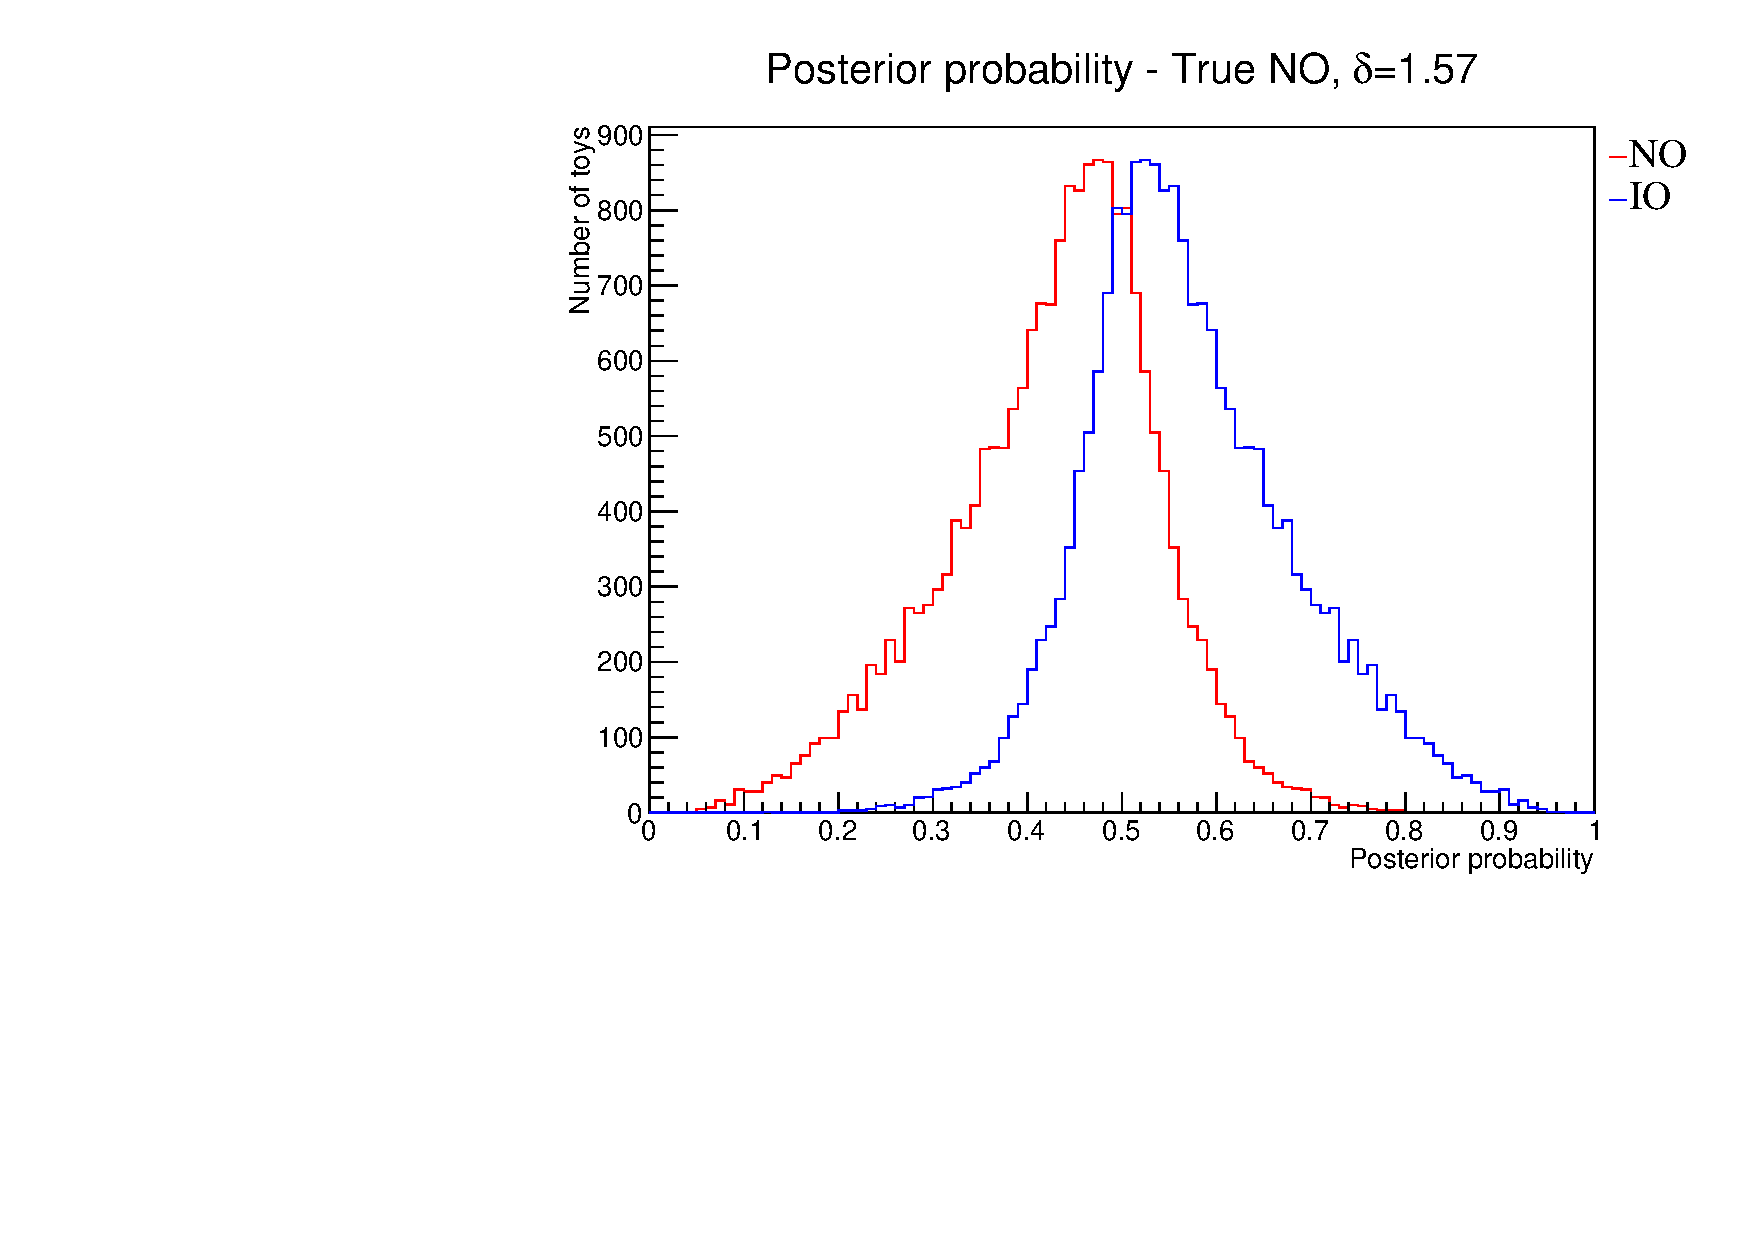
\includegraphics[width=0.9\textwidth, page=1]{images/mh/mh_posterior_ppi2}
		\caption{True normal ordering}
	\end{subfigure}
	\begin{subfigure}[b]{0.49\textwidth}
		\includegraphics[width=0.9\textwidth, page=2]{images/mh/mh_posterior_ppi2}
		\caption{True inverted ordering}
	\end{subfigure}
	\caption {
		Posterior probability distributions of the two mass orderings given $\delta_{CP} = +\pi/2$ and the true mass ordering.
	}
	\label{fig:mh_dcp_ppi2}
\end{figure*}

\begin{table}[htb]
\centering
\begin{tabular}{| c | c | c |}
\hline
True ordering & Reject false ordering & Reject true ordering \\
\hline
Normal & 0.00000 & 0.00010 \\
Inverted & 0.00273 & 0.00000 \\
\hline
\end{tabular}

\caption{
The probability to reject the false and true mass orderings at 95\% threshold for the given true mass ordering.
}
\label{tab:mh_dcp_ppi2}
\end{table}

It can be seen from \cref{tab:mh_dcp_ppi2} that we have little sensitivity to the mass ordering for true $\delta_{CP} = +\pi/2$.

\FloatBarrier

\subsection{Results for $\delta_{CP} = +3\pi/4$}
In \cref{fig:mh_dcp_p3pi4} the mass ordering posterior probability distributions are shown with true $\delta_{CP} = +3\pi/4$ in the case of each true mass ordering, while \cref{tab:mh_dcp_p3pi4} shows the probability of rejecting each mass ordering for a given true mass ordering.

\begin{figure*}[htb]
	\center
	\begin{subfigure}[b]{0.49\textwidth}
		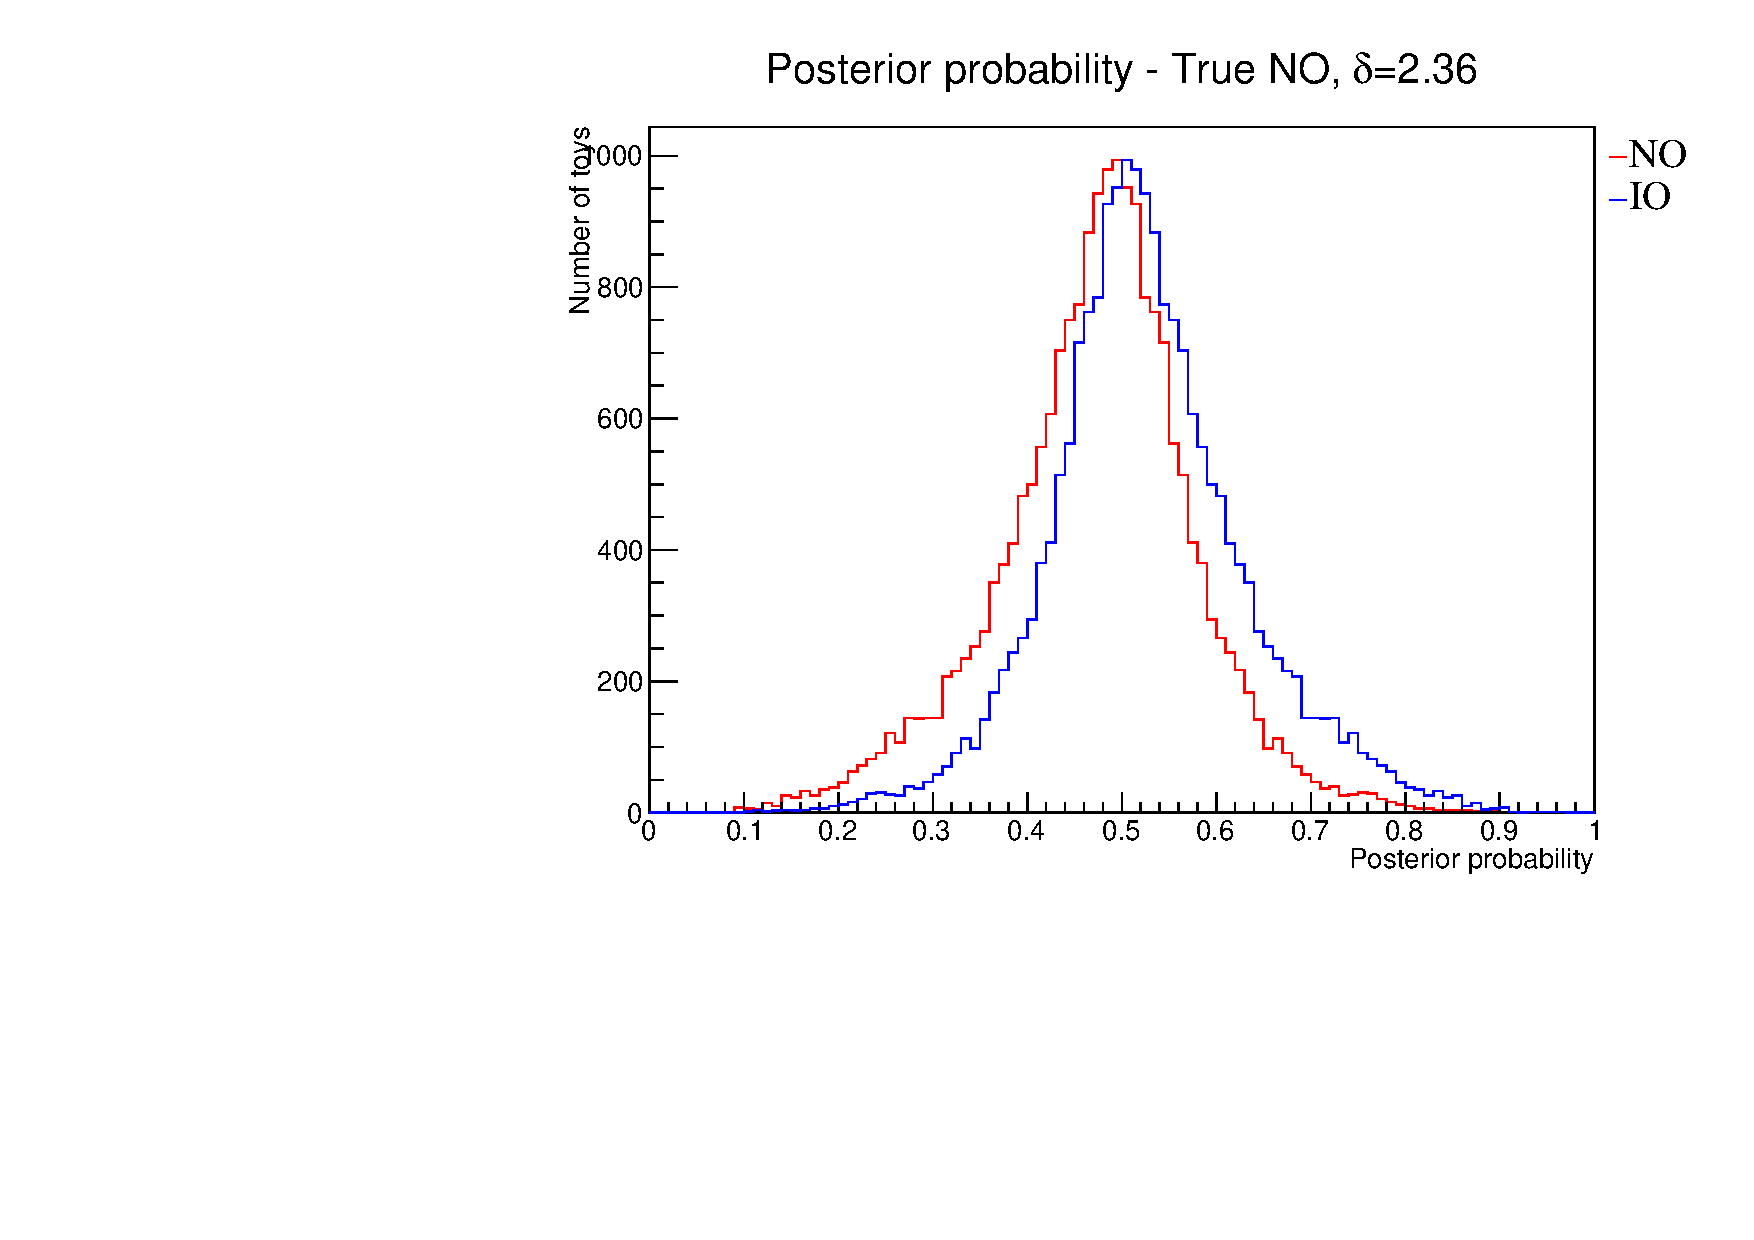
\includegraphics[width=0.9\textwidth, page=1]{images/mh/mh_posterior_p3pi4}
		\caption{True normal ordering}
	\end{subfigure}
	\begin{subfigure}[b]{0.49\textwidth}
		\includegraphics[width=0.9\textwidth, page=2]{images/mh/mh_posterior_p3pi4}
		\caption{True inverted ordering}
	\end{subfigure}
	\caption {
		Posterior probability distributions of the two mass orderings given $\delta_{CP} = +3\pi/4$ and the true mass ordering.
	}
	\label{fig:mh_dcp_p3pi4}
\end{figure*}

\begin{table}[htb]
\centering
\begin{tabular}{| c | c | c |}
\hline
True ordering & Reject false ordering & Reject true ordering \\
\hline
Normal & 0.00000 & 0.00010 \\
Inverted & 0.00090 & 0.00000 \\
\hline
\end{tabular}

\caption{
The probability to reject the false and true mass orderings at 95\% threshold for the given true mass ordering.
}
\label{tab:mh_dcp_p3pi4}
\end{table}

It can be seen from \cref{tab:mh_dcp_p3pi4} that we have little sensitivity to the mass ordering for true $\delta_{CP} = +3\pi/4$.

\FloatBarrier

\subsection{Results for $\delta_{CP} = -1.88$}
In \cref{fig:mh_dcp_bf} the mass ordering posterior probability distributions are shown with true $\delta_{CP} = -1.88$ and true normal ordering (the best-fit from the analysis), along with the posterior probability calculated from the data.

\begin{figure*}[htb]
	\center
	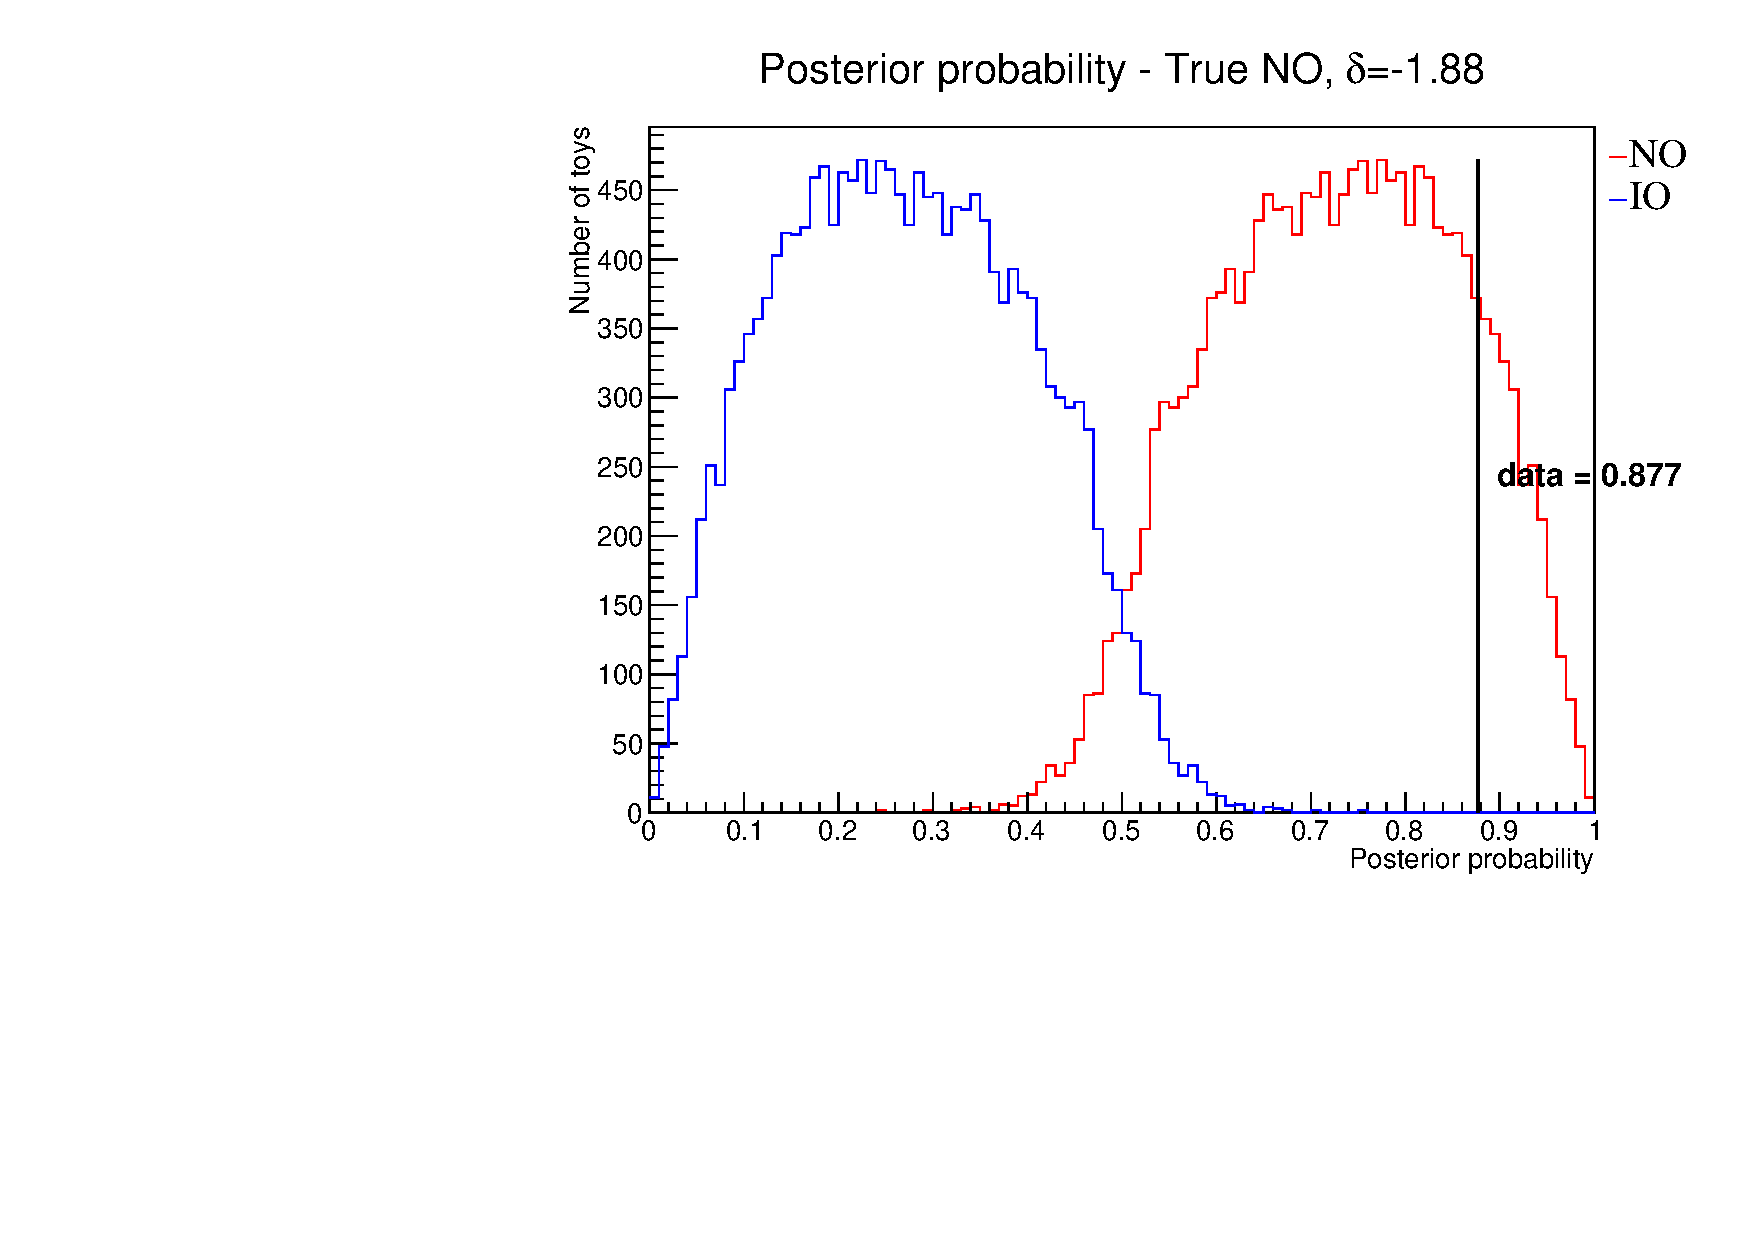
\includegraphics[width=0.8\textwidth, page=1]{images/mh/mh_posterior_bf}
	\caption {
		Posterior probability distributions of the two mass orderings given $\delta_{CP} = -1.88$ and true normal ordering.
	}
	\label{fig:mh_dcp_bf}
\end{figure*}

As expected, the distribution of posterior probabilities for the toys is similar to that of $\delta_{CP} = -\pi/2$, while the posterior probability for normal ordering is 0.877 from the data fits. The integral of the distribution of posterior probabilities to the right of this value yields a $p$-value to reject the inverted ordering of 0.142.

\FloatBarrier

\subsection{Discussion}

For $\delta_{CP} = -\pi/2$ the normal ordering hypothesis is most likely to give a significant result, irrespective of the true mass ordering, with 2.8\% of the NH toys having a posterior probability of at least 0.95 for true normal ordering and 0.1\% of the NH toys having a posterior probability of at least 0.95 for true inverted ordering. Furthermore, the rate at which we reject the true ordering in this case is about 6\% of the rate at which we reject the false hypothesis, appearing consistent with our interpretation of posterior probability; that is given an equal prior probability for each ordering and a posterior probability of 0.95, in about 95\% of the toys the correct ordering is preferred.

For all other tested true values of \deltacp the sensitivity to the mass ordering is limited, with fewer than 1\% of toys rejecting any given mass ordering hypothesis and the ratio of rejections of true and false hypotheses rendered unreliable by very low toy counts in one, or both values.

With respect to the posterior probability computed from data, 14.2\% of the toys generated from the best-fit values of \deltacp and the mass ordering had a posterior probability for normal ordering of at least 0.877.